\section{Experiments}
\label{sec:experiments_reward}

Our experiments aim to answer the following questions: (1) How effectively does our method perform without any prior knowledge of robot embodiment or robot demonstrations? (2) How does our method compare to previous work? (3) Does domain augmentation improve simulation performance? (4) Does our method improve when trained on additional tasks?

\begin{figure}[H]
\centering
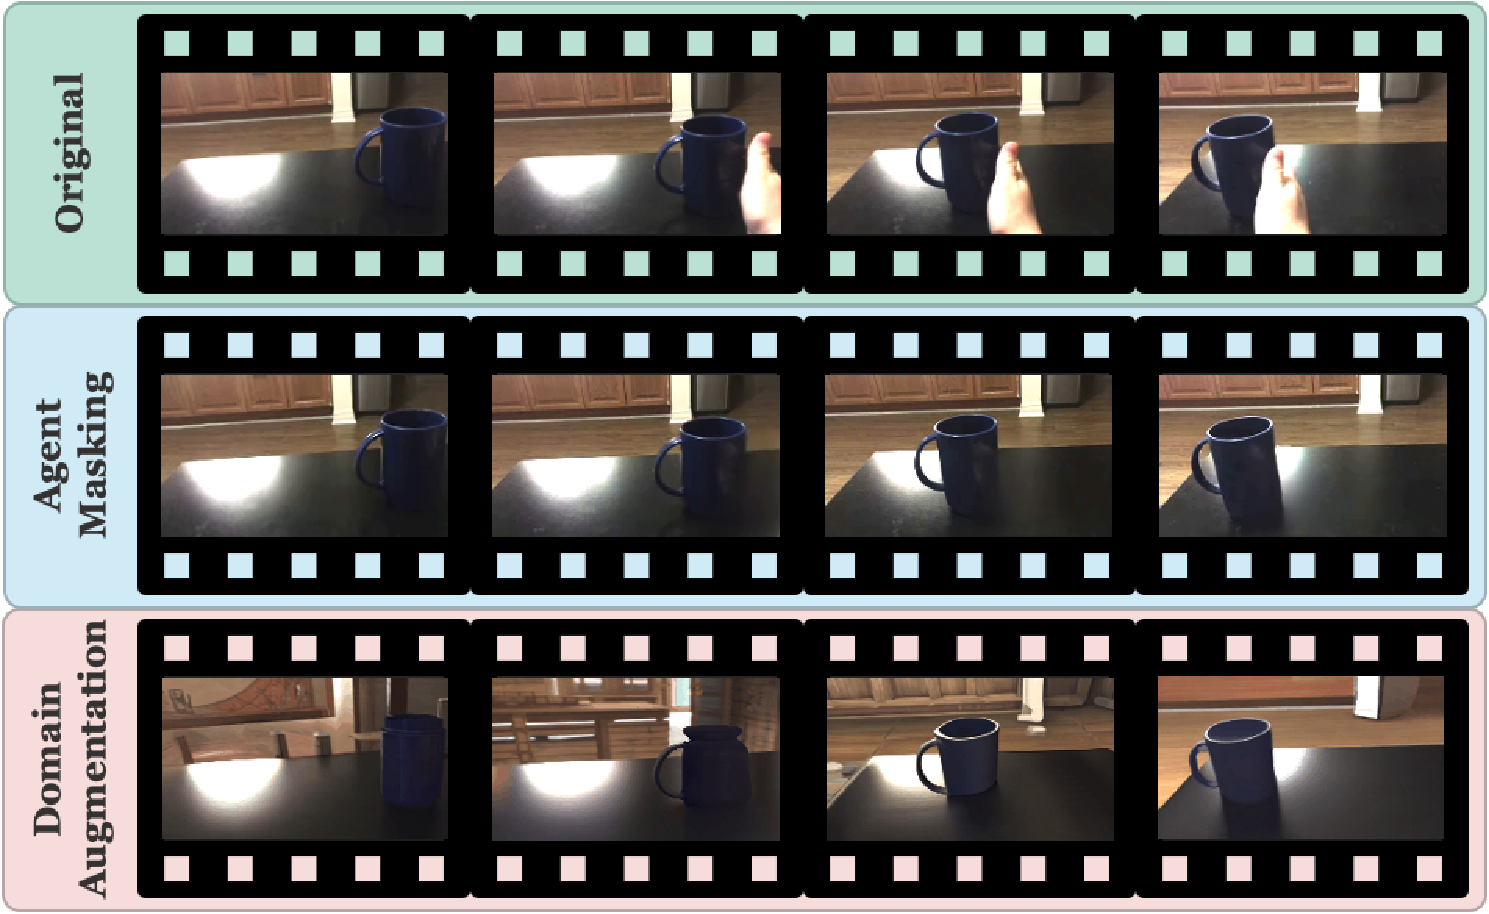
\includegraphics[width=\linewidth]{figs_reward/qual_results.pdf}
\vspace{-0.2in}
   \caption{\small Qualitative Outputs: We show the intermediate results of (1) removing the agent and (2) modifying the background with pre-trained text-to-image models.}
    \label{fig:qual_outputs_reward}
    \vspace{-0.15in}
\end{figure}

\subsection{Comparison to Prior Work}

% First, we wish to answer the following question: \textbf{how does prior work fare when training only on human videos}? In particular, we want to compare methods that learn reward or distance functions and use only human demos at test time.

We use two prior works as baselines: DVD \cite{DVD} and VIP \cite{VIP}. DVD's results involve training on both human and robot videos, so we hypothesize that training only on human videos is not sufficient for learning policies for robots at test time. The DVD reward function does not generalize to unseen robot embodiments. Methods like VIP that pretrain on diverse human datasets generate a reward that represents a distance function to a goal image in the robot's environment. However, we only produce human demonstrations at test time, so we hypothesize this approach will not work well either.

Our results for these baseline methods are in Table \ref{table:baseline_comparison_reward}. The methods we show results for are as follows:

\begin{itemize}
    \item \verb|Shaped Reward|: A human-specified reward function that is manually shaped for each task.
    \item \verb|DVD-HR|: The original implementation of DVD, trained on both human and in-domain robot demonstrations.
    \item \verb|DVD-H|: A modified version of DVD that is limited to training on only human data.
    \item \verb|VIP|: Using VIP with a goal image from an OOD human video at test time.
\end{itemize}

In the first two rows, privileged information is available for the reward function (either a manually shaped reward or robot demonstrations are available). When DVD does not have access to in-domain robot data, there is a significant decline in performance in the zero-shot setting. The DVD model struggles to learn a reward function that can transfer to the robot's environment without robot demonstrations. In practice, we see that it only performs one task, even when given demos of other tasks. VIP also does not perform well because it requires goal image in the robot's setting.

The results of our method are also depicted in Table~\ref{table:baseline_comparison_reward}. We present our method with and without visual domain augmentation. Both reward functions perform strongly on all three tasks despite not having seen the environment in the training data or at test time. Our method performs significantly better than DVD-H and VIP in the zero-shot setting. Our method even outperforms DVD-HR on two of the three tasks. Overall, we believe that removing the agent encourages the representations learned by our method to more accurately match the functional meaning of the task by focusing on the changes in the environment. Accordingly, our method can perform better than models like DVD-HR.

\begin{table}[t]
    \centering
    \resizebox{\linewidth}{!}
    {%
        \begin{tabular}{lcccc}
        \toprule
        Model & Close Drawer & Push Mug Away & Move Mug Right & Average \\
        \midrule\midrule
        Shaped Reward & 0.99 & 0.95 & 0.99 & 0.98 \\
        DVD-HR \cite{DVD} & 0.75 & 0.59 & 0.06 & 0.47 \\
        \midrule
        \textit{Human-only Reward Functions}: \\
        DVD-H \cite{DVD} & 0.0 & 0.62 & 0.0 & 0.21 \\
        VIP \cite{VIP} & 0.09 & 0.22 & 0.14 & 0.15 \\
        \midrule
        Ours & 0.65 & 0.96 & 0.75 & 0.79 \\
        Ours + Domain Augmentation & 0.84 & 0.96 & 0.88 & 0.89 \\
        \bottomrule
        \end{tabular}
    }
    \vspace{0.05in}
    \caption{Fraction of successful iterations for each model with varying data used at training and test time. Each model was averaged over 10 different seeds, each seed being run for 100 CEM iterations.}
    \label{table:baseline_comparison_reward}
\end{table}

\subsection{Effect of visual domain augmentation}

As shown in Table~\ref{table:baseline_comparison_reward}, domain augmentation with Stable Diffusion improves the results of our method on two of the three tasks. Overall, it has an 89\% success rate while our method without augmentation has a success rate of 79\%. With domain augmentation, our method beats DVD-HR in all three tasks and is moving closer to the performance of the shaped reward. Our method with domain augmentation performs the zero-shot baselines by 68\%. Even though Stable Diffusion is not trained on robotics-related data, it is able to provide meaningful priors to enhance training and potentially improve generalization.

More aggressive augmentation could potentially improve the amount of generalization, but could also reduce the temporal consistency of the video as a whole. For sample augmentation outputs, see Figure~\ref{fig:qual_outputs_reward}.

\subsection{Number of Training Tasks}

\begin{figure}[t]
\vspace{-0.2in}
\begin{center}
    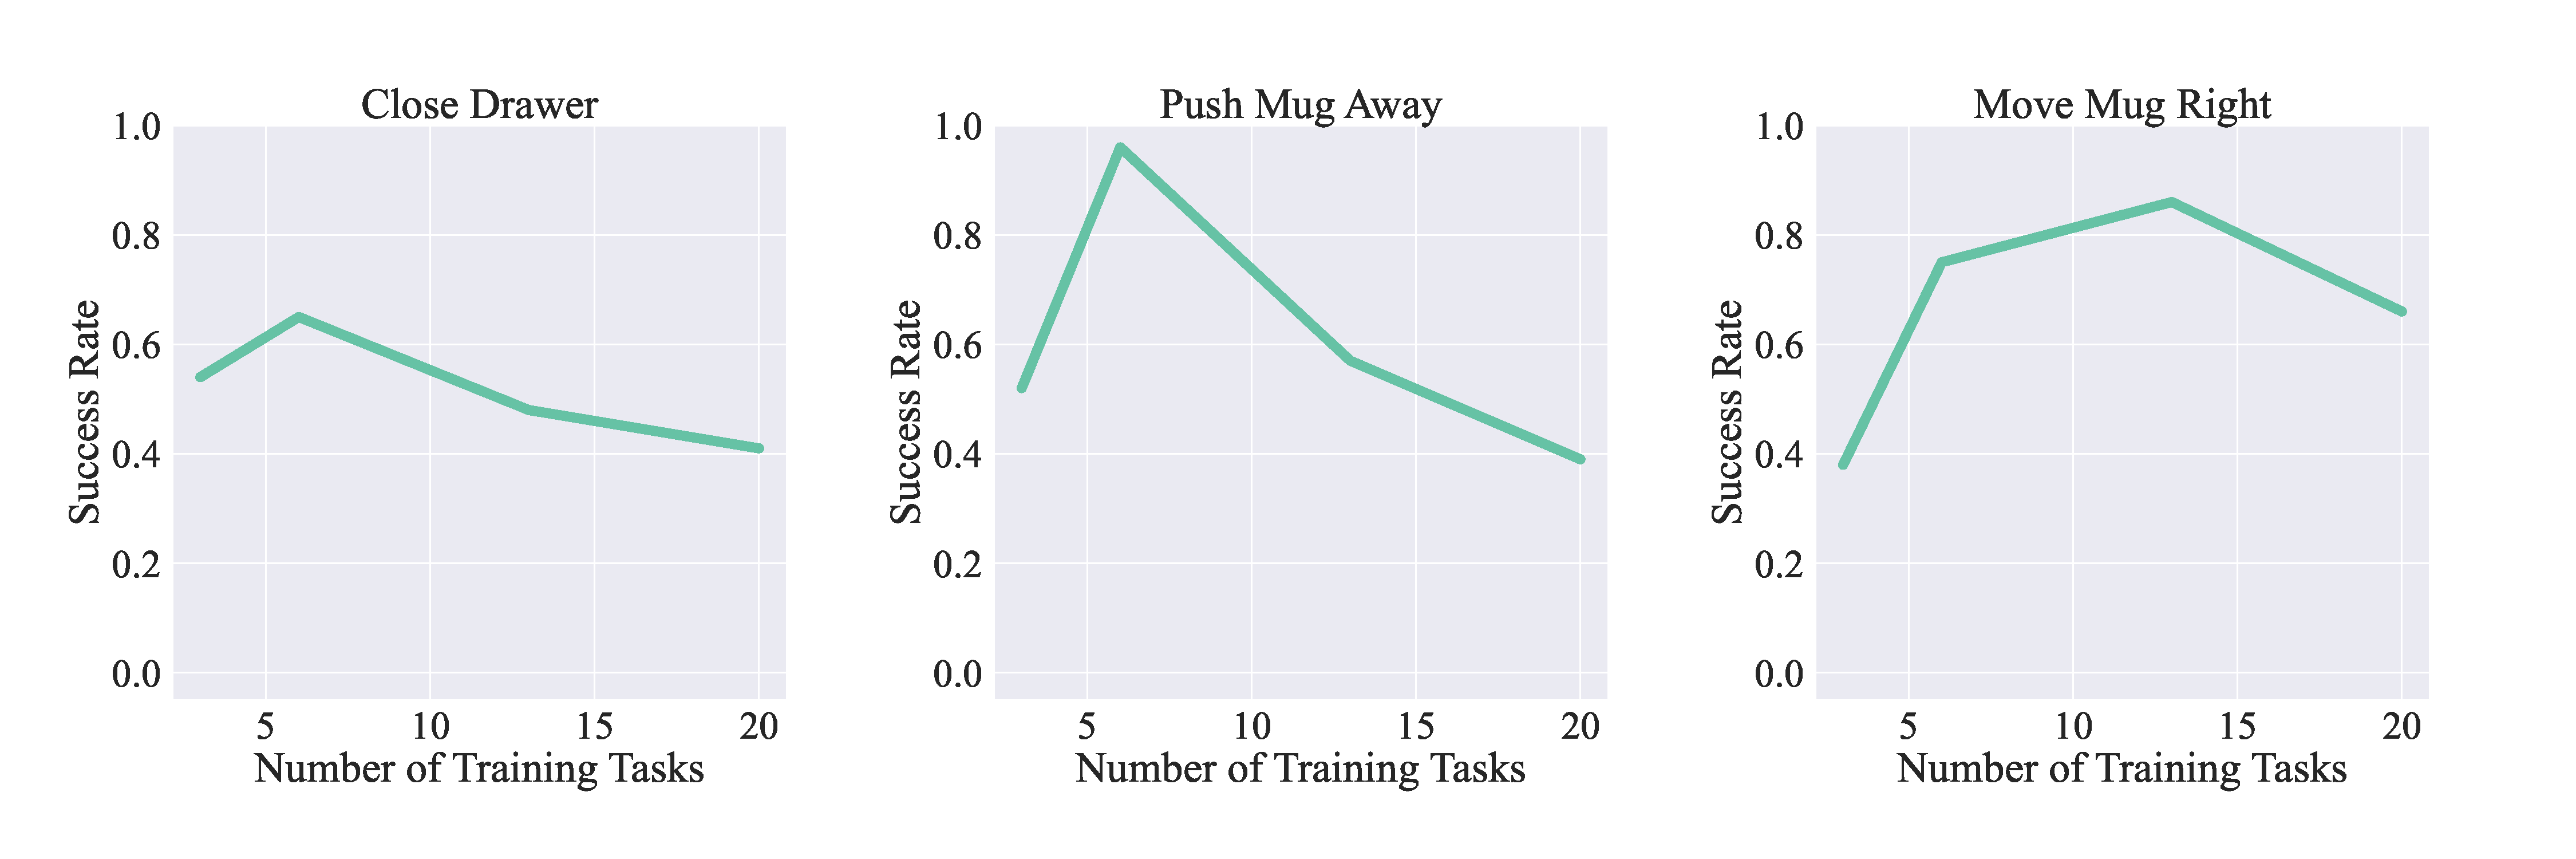
\includegraphics[width=\linewidth]{figs_reward/graph_task_ablation.pdf}
\end{center}
\vspace{-0.1in}
  \caption{\small We investigate how adding unrelated tasks in training affects the downstream performance of our method.}
 \label{fig:graph_task_ablation_reward}
\end{figure}

\begin{table}[t]
    \centering
    \resizebox{\linewidth}{!}
    {%
        \begin{tabular}{lcc}
        \toprule
        Task & Our Method (6 Task Training) & Our Method (20 Task Training) \\
        \midrule
        Close Drawer & 0.65 & 0.41 \\
        Push Mug Away & 0.96 & 0.39 \\
        Move Mug Right & 0.75 & 0.66 \\
        Move Mug Left & 0.65 & 0.31 \\
        Pull Mug to Camera & 0.01 & 0.06 \\
        Open Drawer & 0.25 & 0.0 \\
        \midrule\midrule
        Average & 0.55 & 0.31 \\
        \bottomrule
        \end{tabular}
    }
    \vspace{0.05in}
    \caption{Fraction successful iterations for reward models trained with varying number of tasks.}
    \label{table:more_tasks_reward}
\end{table}


The results that we described in the previous section involve training on 6 tasks. One question we wish to answer is how does the number of tasks we train on affect the performance of the reward function on robotic tasks? In other words, how does the diversity of the training data affect the quality of the reward function learned, and do unrelated videos enhance the reward function learned?

To investigate this, we additionally train a reward function with our method with 3 tasks, 13 tasks, and 20 tasks. All of these variations include the three evaluation tasks in the training set. We evaluate the 4 reward functions with the three original evaluation tasks. We show these results in Figure~\ref{fig:graph_task_ablation_reward}. We also show results comparing our method with 6 task training and 20 task training on 3 additional evaluation tasks in Table~\ref{table:more_tasks_reward}.

Based on the results in Figure~\ref{fig:graph_task_ablation_reward}, we find that scaling to more tasks in training produces better performance and generalization up to a point. Perhaps the reason the 3-task model performs worse than the 6-task reward function is that there are fewer total videos for training. While both models are trained for the same number of epochs, the number of videos in each epoch is smaller for the model trained with three tasks.

However, after 6 tasks, the success rate plateaus and decreases when going to 13 and then 20 training tasks. This is reflected even more in Table~\ref{table:more_tasks_reward} where the 20-task model performs worse on all 6 evaluation tasks. This is probably due to the structure of the reward model: as the discriminator needs to be able to distinguish between more tasks, it might struggle to disambiguate the salient features for the evaluation tasks compared to the other tasks it is trained on. As a result, our method loses robustness when training on \textit{too many} unrelated tasks.
